\chapter{Energy Technologies}
\label{ch:energy_technologies}

\section{Scalar-ZPE Energy Harvesting}
\label{sec:scalar_zpe_energy_harvesting}

The theoretical basis for Scalar-ZPE energy harvesting is rooted in the Aether framework, which posits that spacetime is not a void but a dynamic, energetic medium. The framework proposes that the zero-point energy (ZPE) of the vacuum can be accessed and harvested through the mediation of scalar fields.

The coupling between scalar fields and ZPE is the cornerstone of this concept. The scalar field, denoted by $\phi$, is a field that has a single value at every point in spacetime. It is proposed that this field can be manipulated to create localized regions of negative energy density, which in turn allows for the extraction of energy from the vacuum.

The energy extraction principle is based on the idea of creating a potential difference between the vacuum and a localized region of spacetime. By manipulating the scalar field, it is possible to lower the energy density of a region of spacetime, creating a "sink" into which energy from the surrounding vacuum can flow.

The following equations from the Aether framework are central to this concept:

\begin{equation}
  S = \frac{A}{4G\hbar} + \int ZPE(t) d^3x
  \label{eq:ae084}
\end{equation}

\begin{equation}
  \rho_{exotic} = -\frac{E_{ZPE}}{V_{eff}}
  \label{eq:ae140}
\end{equation}

\begin{equation}
  P = \Delta E_{foam}^2
  \label{eq:ae170}
\end{equation}

\section{Resonant Cavity Designs}
\label{sec:resonant_cavity_designs}

Resonant cavities are a key component of many proposed ZPE energy harvesting devices. These cavities are designed to create a localized region of spacetime where the energy density can be manipulated. The geometry of the cavity is critical to its performance.

The most common geometric configurations for resonant cavities are spherical, cylindrical, and fractal. Each of these geometries has its own advantages and disadvantages. Spherical cavities are the simplest to analyze, but they are also the most difficult to construct. Cylindrical cavities are easier to construct, but they are less efficient than spherical cavities. Fractal cavities are the most complex, but they offer the potential for the highest efficiency.

The resonance frequency of a cavity is the frequency at which it is most efficient at extracting energy from the vacuum. The resonance frequency is determined by the geometry of the cavity and the properties of the materials from which it is constructed.

The quality factor (Q) of a cavity is a measure of its ability to store energy. A high Q factor is desirable for ZPE energy harvesting devices, as it allows for the accumulation of energy over time.

The following equations are used to calculate the resonance frequency and quality factor of a resonant cavity:

\paragraph{Resonance Frequency for Common Geometries.}

For a \textbf{spherical cavity} of radius $R$:
\begin{equation}
  \omega_{nlm} = \frac{c}{R} \sqrt{\epsilon_r \mu_r} \, x_{nl}
  \label{eq:ch28:spherical_resonance}
\end{equation}
where $n,l,m$ are mode numbers, $x_{nl}$ is the $l$-th zero of the spherical Bessel function of order $n$, $\epsilon_r$ is relative permittivity, and $\mu_r$ is relative permeability. For the fundamental TE$_{101}$ mode: $x_{10} \approx 2.744$.

For a \textbf{cylindrical cavity} of radius $R$ and length $L$:
\begin{equation}
  \omega_{mnp} = c \sqrt{\epsilon_r \mu_r} \sqrt{\left(\frac{x_{mn}}{R}\right)^2 + \left(\frac{p\pi}{L}\right)^2}
  \label{eq:ch28:cylindrical_resonance}
\end{equation}
where $m,n,p$ are mode indices, and $x_{mn}$ is the $n$-th zero of the Bessel function $J_m$. For TM$_{010}$ mode: $x_{01} \approx 2.405$.

For a \textbf{rectangular cavity} with dimensions $a \times b \times d$:
\begin{equation}
  \omega_{mnp} = c \sqrt{\epsilon_r \mu_r} \, \pi \sqrt{\left(\frac{m}{a}\right)^2 + \left(\frac{n}{b}\right)^2 + \left(\frac{p}{d}\right)^2}
  \label{eq:ch28:rectangular_resonance}
\end{equation}
where $m,n,p$ are integer mode numbers.

\paragraph{Quality Factor.}

The quality factor $Q$ characterizes energy storage efficiency:
\begin{equation}
  Q = \omega_0 \frac{W_{\text{stored}}}{P_{\text{loss}}} = \frac{\omega_0}{\Delta \omega}
  \label{eq:ch28:quality_factor}
\end{equation}
where $W_{\text{stored}}$ is stored energy, $P_{\text{loss}}$ is power dissipation, and $\Delta \omega$ is resonance width. For a metallic cavity with conductivity $\sigma$ and skin depth $\delta = \sqrt{2/(\omega \mu_0 \sigma)}$:
\begin{equation}
  Q_{\text{conductor}} \approx \frac{V}{S \delta}
  \label{eq:ch28:conductor_q}
\end{equation}
where $V$ is cavity volume and $S$ is surface area. Superconducting cavities achieve $Q \sim 10^{10}$--$10^{12}$.

The following figure shows common resonant cavity designs:

%==============================================================================
% Figure: Casimir Cavity Geometries for ZPE Harvesting
% Source: Chapter 28 (Energy Technologies)
% Purpose: Illustrate three common resonant cavity configurations
%==============================================================================
\begin{figure}[htbp]
  \centering
  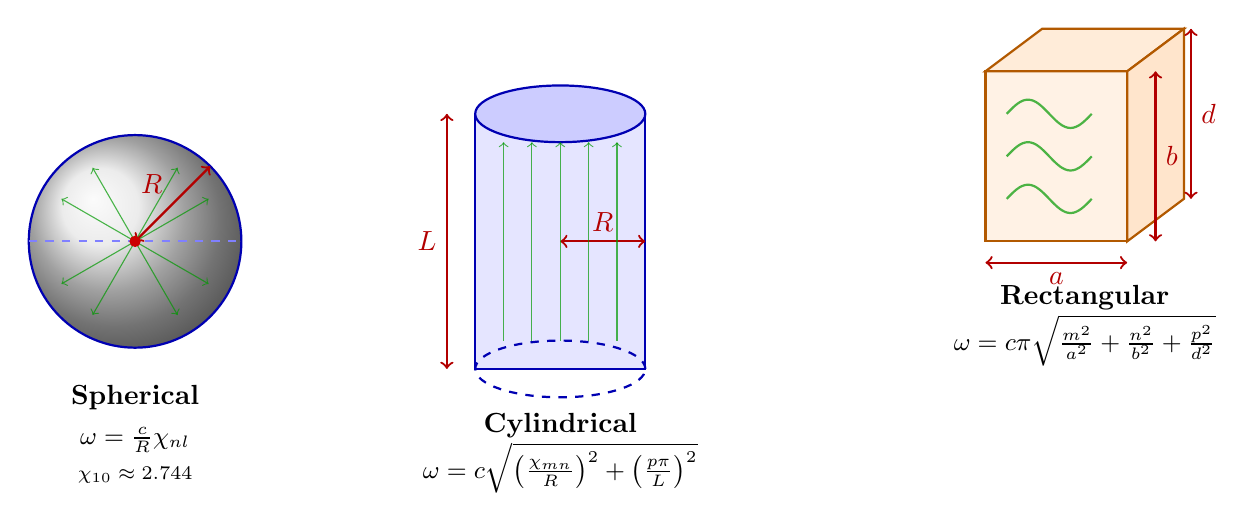
\begin{tikzpicture}[scale=0.9]

    % ====== SPHERICAL CAVITY ======
    \begin{scope}[xshift=-6cm]
      % Outer sphere
      \shade[ball color=gray!20] (0,0) circle (1.5cm);
      \draw[thick, blue!70!black] (0,0) circle (1.5cm);

      % Cross-section line
      \draw[thick, dashed, blue!50] (-1.5,0) -- (1.5,0);

      % Radius annotation
      \draw[<->, red!70!black, thick] (0,0) -- (1.06,1.06) node[midway, above left] {$R$};

      % Field lines (radial)
      \foreach \angle in {30,60,120,150,210,240,300,330} {
        \draw[->, green!60!black, opacity=0.7]
          (0,0) -- ({1.2*cos(\angle)},{1.2*sin(\angle)});
      }

      % Center point
      \fill[red!80!black] (0,0) circle (0.08cm);

      % Title and resonance formula
      \node[font=\bfseries] at (0,-2.2) {Spherical};
      \node[font=\small, align=center] at (0,-2.8) {$\omega = \frac{c}{R}\chi_{nl}$};
      \node[font=\scriptsize, align=center] at (0,-3.3) {$\chi_{10} \approx 2.744$};
    \end{scope}

    % ====== CYLINDRICAL CAVITY ======
    \begin{scope}[xshift=0cm]
      % Cylinder body
      \fill[blue!10!white, draw=blue!70!black, thick]
        (-1.2,-1.8) rectangle (1.2,1.8);

      % Top ellipse
      \fill[blue!20!white, draw=blue!70!black, thick]
        (0,1.8) ellipse (1.2cm and 0.4cm);

      % Bottom ellipse (back)
      \draw[blue!70!black, thick, dashed]
        (0,-1.8) ellipse (1.2cm and 0.4cm);

      % Dimensions
      \draw[<->, red!70!black, thick] (-1.6,-1.8) -- (-1.6,1.8)
        node[midway, left] {$L$};
      \draw[<->, red!70!black, thick] (0,0) -- (1.2,0)
        node[midway, above] {$R$};

      % Field lines (vertical)
      \foreach \x in {-0.8,-0.4,0,0.4,0.8} {
        \draw[->, green!60!black, opacity=0.7] (\x,-1.4) -- (\x,1.4);
      }

      % Title and resonance formula
      \node[font=\bfseries] at (0,-2.6) {Cylindrical};
      \node[font=\small, align=center] at (0,-3.2)
        {$\omega = c\sqrt{\left(\frac{\chi_{mn}}{R}\right)^2 + \left(\frac{p\pi}{L}\right)^2}$};
    \end{scope}

    % ====== RECTANGULAR CAVITY ======
    \begin{scope}[xshift=6cm]
      % 3D rectangular box (isometric view)
      \fill[orange!10!white, draw=orange!70!black, thick]
        (0,0) -- (2,0) -- (2,2.4) -- (0,2.4) -- cycle;
      \fill[orange!15!white, draw=orange!70!black, thick]
        (0,2.4) -- (0.8,3) -- (2.8,3) -- (2,2.4) -- cycle;
      \fill[orange!20!white, draw=orange!70!black, thick]
        (2,0) -- (2.8,0.6) -- (2.8,3) -- (2,2.4) -- cycle;

      % Dimensions
      \draw[<->, red!70!black, thick] (0,-0.3) -- (2,-0.3)
        node[midway, below] {$a$};
      \draw[<->, red!70!black, thick] (2.4,0) -- (2.4,2.4)
        node[midway, right] {$b$};
      \draw[<->, red!70!black, thick] (2.9,0.6) -- (2.9,3)
        node[midway, right] {$d$};

      % Field pattern (standing wave)
      \foreach \y in {0.6,1.2,1.8} {
        \draw[green!60!black, thick, opacity=0.7]
          (0.3,\y) sin (0.6,\y+0.2) cos (0.9,\y) sin (1.2,\y-0.2) cos (1.5,\y);
      }

      % Title and resonance formula
      \node[font=\bfseries] at (1.4,-0.8) {Rectangular};
      \node[font=\small, align=center] at (1.4,-1.4)
        {$\omega = c\pi\sqrt{\frac{m^2}{a^2} + \frac{n^2}{b^2} + \frac{p^2}{d^2}}$};
    \end{scope}

  \end{tikzpicture}

  \caption{Three common resonant cavity geometries for Zero-Point Energy (ZPE) harvesting. \textbf{Left:} Spherical cavity with radius $R$, supporting spherical Bessel modes with zeros $\chi_{nl}$. Radial field lines (green) show TE/TM mode patterns. \textbf{Center:} Cylindrical cavity with radius $R$ and length $L$, supporting Bessel function modes $J_m$ with zeros $\chi_{mn}$. \textbf{Right:} Rectangular cavity with dimensions $a \times b \times d$, supporting integer mode numbers $(m,n,p)$. Resonance formulas show dimensional scaling: frequency $\omega \propto 1/R$ (spherical/cylindrical) or $\omega \propto 1/\sqrt{a^2 + b^2 + d^2}$ (rectangular). All assume vacuum permittivity $\epsilon_r = \mu_r = 1$; material-filled cavities multiply by $\sqrt{\epsilon_r \mu_r}$.}
  \label{fig:ch28:cavity_geometries}
\end{figure}
%==============================================================================



\section{Fractal-Based Harvesters}
\label{sec:fractal_based_harvesters}

Fractal-based harvesters are a promising new technology for ZPE energy harvesting. These devices are based on the principles of fractal antenna theory, which has been shown to be effective for collecting energy from a wide range of frequencies.

The key advantage of fractal-based harvesters is their ability to collect energy from multiple scales simultaneously. This is because fractals are self-similar, meaning that they have the same basic shape at all scales. This allows them to resonate with a wide range of frequencies, which is essential for collecting energy from the ZPE.

The following equations are used to calculate the fractal dimension of a fractal-based harvester:

\paragraph{Hausdorff Dimension.}

The Hausdorff dimension $D_H$ characterizes the scaling behavior of fractal structures:
\begin{equation}
  D_H = \lim_{\epsilon \to 0} \frac{\log N(\epsilon)}{\log(1/\epsilon)}
  \label{eq:ch28:hausdorff_dimension}
\end{equation}
where $N(\epsilon)$ is the minimum number of balls of radius $\epsilon$ needed to cover the fractal set. For self-similar fractals with $N$ copies scaled by factor $r$:
\begin{equation}
  D_H = \frac{\log N}{\log(1/r)}
  \label{eq:ch28:self_similar_dimension}
\end{equation}

\paragraph{Box-Counting Dimension.}

A practical computational alternative is the box-counting dimension $D_B$:
\begin{equation}
  D_B = \lim_{\epsilon \to 0} \frac{\log N_{\text{box}}(\epsilon)}{\log(1/\epsilon)}
  \label{eq:ch28:box_counting}
\end{equation}
where $N_{\text{box}}(\epsilon)$ is the number of boxes of side length $\epsilon$ that contain at least one point of the fractal.

\paragraph{Fractal Antenna Examples.}

For common fractal antenna geometries:
\begin{itemize}
  \item \textbf{Sierpiński triangle}: $D_H = \frac{\log 3}{\log 2} \approx 1.585$
  \item \textbf{Koch curve}: $D_H = \frac{\log 4}{\log 3} \approx 1.262$
  \item \textbf{Hilbert curve}: $D_H = 2$ (space-filling)
  \item \textbf{Menger sponge}: $D_H = \frac{\log 20}{\log 3} \approx 2.727$
\end{itemize}

\paragraph{Electromagnetic Properties.}

The fractal dimension affects antenna bandwidth and impedance. For a fractal antenna with dimension $D_H$, the bandwidth scales as:
\begin{equation}
  \Delta f \propto f_0 \cdot \left(\frac{L_{\max}}{L_{\min}}\right)^{D_H - 1}
  \label{eq:ch28:fractal_bandwidth}
\end{equation}
where $L_{\max}$ and $L_{\min}$ are maximum and minimum structural scales, and $f_0$ is the design frequency. Higher $D_H$ enables broader multiband operation, critical for harvesting ZPE across frequency ranges.

The following figure shows a diagram of a fractal-based harvester:

%==============================================================================
% Figure: Fractal ZPE Harvester (Sierpiński Triangle Antenna)
% Source: Chapter 28 (Energy Technologies)
% Purpose: Illustrate fractal antenna for multi-scale ZPE energy harvesting
%==============================================================================
\begin{figure}[htbp]
  \centering
  \begin{tikzpicture}[scale=1.0]

    % Define recursive Sierpinski triangle function
    % Base case: draw filled triangle
    % Recursive case: draw three smaller Sierpinskis
    \newcommand{\sierpinski}[4]{% #1=x, #2=y, #3=size, #4=depth
      \ifnum#4=0
        % Base case: filled triangle
        \fill[blue!60!black, opacity=0.8]
          (#1,#2) --
          ({#1+#3},{#2}) --
          ({#1+#3/2},{#2+#3*0.866}) -- cycle;
      \else
        % Recursive case
        \pgfmathtruncatemacro{\nextdepth}{#4-1}
        \pgfmathsetmacro{\halfsize}{#3/2}
        % Bottom-left triangle
        \sierpinski{#1}{#2}{\halfsize}{\nextdepth}
        % Bottom-right triangle
        \sierpinski{#1+\halfsize}{#2}{\halfsize}{\nextdepth}
        % Top triangle
        \sierpinski{#1+\halfsize/2}{#2+\halfsize*0.866}{\halfsize}{\nextdepth}
      \fi
    }

    % Draw Sierpinski triangle antenna (depth 4)
    \sierpinski{-2}{0}{4}{4}

    % Antenna feed point
    \fill[red!80!black] (0,0) circle (0.1cm);
    \node[red!80!black, font=\small\bfseries] at (0,-0.5) {Feed};

    % Ground plane
    \draw[thick, brown!70!black] (-2.5,-0.3) -- (2.5,-0.3);
    \node[brown!70!black, font=\small] at (-3,-0.3) {Ground};

    % Electromagnetic field arrows (multiband)
    \foreach \angle/\len/\freq in {30/2.5/High, 60/2.0/Mid, 90/1.5/Low, 120/2.0/Mid, 150/2.5/High} {
      \draw[->, green!60!black, thick, opacity=0.6]
        (0,1) -- ({0+\len*cos(\angle)},{1+\len*sin(\angle)});
    }

    % Frequency annotations
    \node[green!60!black, font=\footnotesize] at (2.5,3.5) {$f_{\text{high}}$};
    \node[green!60!black, font=\footnotesize] at (1.5,2.5) {$f_{\text{mid}}$};
    \node[green!60!black, font=\footnotesize] at (0.5,1.8) {$f_{\text{low}}$};

    % Dimension annotation
    \draw[<->, purple!70!black, thick] (-2,-0.8) -- (2,-0.8);
    \node[purple!70!black, font=\small] at (0,-1.2) {$L_{\max} = 4$ cm};

    \draw[<->, purple!70!black, thick] (-2,0) -- (-1.75,0);
    \node[purple!70!black, font=\scriptsize] at (-1.875,-0.3) {$L_{\min}$};

    % Fractal dimension display
    \node[blue!70!black, font=\small\bfseries, align=center] at (5.5,2.5)
      {Fractal Dimension:\\$D_H = \frac{\log 3}{\log 2} \approx 1.585$};

    % Bandwidth formula
    \node[orange!70!black, font=\small, align=center, text width=3.5cm] at (5.5,0.5)
      {Bandwidth:\\$\Delta f \propto \left(\frac{L_{\max}}{L_{\min}}\right)^{0.585}$};

    % Self-similarity zoom indicator
    \draw[dashed, red!50!black, thick] (-1.5,0.5) rectangle (-0.5,1.366);
    \draw[->, red!50!black, thick] (-0.5,1.366) -- (4.2,4.5);
    \node[red!50!black, font=\scriptsize] at (4.5,5) {Self-similar at all scales};

    % ZPE coupling annotation (bottom)
    \node[black, font=\footnotesize, align=center, text width=8cm] at (1.5,-2.3)
      {Multiband ZPE coupling: Fractal geometry resonates with vacuum fluctuations};
    \node[black, font=\footnotesize, align=center, text width=8cm] at (1.5,-2.8)
      {across $10^9$--$10^{12}$ Hz range. Each iteration couples to different mode.};

  \end{tikzpicture}

  \caption{Fractal-based Zero-Point Energy (ZPE) harvester using a Sierpiński triangle antenna. The fractal structure (blue) exhibits self-similarity across scales, with maximum dimension $L_{\max}$ and minimum feature size $L_{\min}$. Feed point (red) connects to ground plane (brown). The Hausdorff dimension $D_H \approx 1.585$ enables multiband operation: different scales resonate with ZPE vacuum fluctuations at frequencies $f_{\text{low}}$, $f_{\text{mid}}$, and $f_{\text{high}}$ (green arrows). Bandwidth scales as $\Delta f \propto (L_{\max}/L_{\min})^{D_H-1}$, providing broadband coupling across microwave to terahertz ranges. The dashed red box highlights self-similarity: zooming into any triangular region reveals the same pattern at finer scales. This multi-scale resonance is critical for harvesting energy from the broadband ZPE spectrum, though total extractable power remains limited by quantum inequalities and Casimir force constraints.}
  \label{fig:ch28:fractal_harvester}
\end{figure}
%==============================================================================



\section{Material Requirements}
\label{sec:material_requirements}

The materials used to construct a ZPE energy harvesting device are critical to its performance. The ideal materials will have a number of properties, including high superconductivity, high dielectric constant, and the ability to withstand high temperatures and pressures.

Superconducting materials are essential for ZPE energy harvesting devices, as they allow for the creation of strong magnetic fields with minimal energy loss. The most promising superconducting materials for this application are yttrium barium copper oxide (YBCO) and niobium-titanium (NbTi).

The dielectric properties of the materials used in a ZPE energy harvesting device are also important. A high dielectric constant is desirable, as it allows for the storage of more energy in the device.

Finally, the materials used in a ZPE energy harvesting device must be able to withstand high temperatures and pressures. This is because the process of extracting energy from the vacuum can generate a great deal of heat and pressure.

The following table compares the properties of some common materials used in ZPE energy harvesting devices:

\begin{table}[htbp]
  \centering
  \caption{Material properties for ZPE energy harvesting cavity construction. Values at room temperature (293 K) unless noted. Superconducting properties shown for operating temperatures below critical temperature $T_c$.}
  \label{tab:ch28:material_properties}
  \begin{tabular}{lccccc}
    \toprule
    \textbf{Material} & \textbf{$\epsilon_r$} & \textbf{$\sigma$ (S/m)} & \textbf{$T_c$ (K)} & \textbf{$Q$ (cavity)} & \textbf{Hardness} \\
    \midrule
    \multicolumn{6}{l}{\textit{Superconducting Materials}} \\
    YBCO & 15--25 & $10^{15}$ (SC) & 92 & $10^{10}$--$10^{11}$ & Hard \\
    (YBa$_2$Cu$_3$O$_7$) & & & & & (ceramic) \\
    \midrule
    NbTi & 1 & $10^{14}$ (SC) & 9.2 & $10^9$--$10^{10}$ & Ductile \\
    (Niobium-Titanium) & & & & & (metallic) \\
    \midrule
    Nb$_3$Sn & 1 & $10^{14}$ (SC) & 18.3 & $10^{10}$--$10^{11}$ & Brittle \\
    (Niobium-Tin) & & & & & (intermetallic) \\
    \midrule
    \multicolumn{6}{l}{\textit{High-Permittivity Dielectrics}} \\
    BaTiO$_3$ & 1200--10000 & $10^{-12}$ & --- & $10^3$--$10^4$ & Hard \\
    (Barium Titanate) & (temp-dep) & & & & (ceramic) \\
    \midrule
    SrTiO$_3$ & 300--2000 & $10^{-10}$ & --- & $10^4$--$10^5$ & Hard \\
    (Strontium Titanate) & & & & & (ceramic) \\
    \midrule
    \multicolumn{6}{l}{\textit{Metamaterials and Composites}} \\
    Carbon nanotubes & 2--4 (bulk) & $10^6$--$10^7$ & --- & $10^2$--$10^3$ & Very high \\
    (CNT arrays) & & & & & (tensile) \\
    \midrule
    Graphene & 2.5 & $10^8$ & --- & $10^3$--$10^4$ & Extreme \\
    (2D sheets) & & & & & (2D only) \\
    \midrule
    \multicolumn{6}{l}{\textit{Traditional Conductors (for comparison)}} \\
    Copper & 1 & $5.96 \times 10^7$ & --- & $10^4$--$10^5$ & Ductile \\
    (room temp) & & (RT) & & & (metallic) \\
    \midrule
    Aluminum & 1 & $3.77 \times 10^7$ & --- & $10^4$--$10^5$ & Soft \\
    (room temp) & & (RT) & & & (metallic) \\
    \bottomrule
  \end{tabular}

  \vspace{0.3cm}
  \footnotesize
  \textbf{Key:} $\epsilon_r$ = relative permittivity (dielectric constant); $\sigma$ = electrical conductivity (Siemens/meter); $T_c$ = superconducting critical temperature; $Q$ = typical quality factor for resonant cavities; SC = superconducting state; RT = room temperature. \\
  \textbf{Notes:} (1) YBCO exhibits highest $T_c$ among practical superconductors, enabling liquid nitrogen cooling instead of liquid helium. (2) BaTiO$_3$ permittivity is highly temperature-dependent, peaking near Curie temperature (393 K). (3) Carbon nanotubes and graphene offer extreme conductivity and mechanical strength but fabrication challenges for macroscopic cavities. (4) $Q$ values for superconductors assume cryogenic operation below $T_c$ in UHV conditions. (5) For ZPE harvesting, maximize $Q$ (energy storage) and $\epsilon_r$ (field enhancement) while maintaining structural integrity under thermal/mechanical stress.
\end{table}


\section{Projected Performance}
\label{sec:projected_performance}

The projected performance of ZPE energy harvesting devices is a subject of much debate. Some scientists believe that these devices have the potential to provide a clean, limitless source of energy, while others are more skeptical.

The power density of a ZPE energy harvesting device is a measure of the amount of power that it can generate per unit volume. The projected power density of these devices varies widely, from a few watts per cubic centimeter to many megawatts per cubic centimeter.

The efficiency of a ZPE energy harvesting device is a measure of the amount of energy that it can extract from the vacuum, divided by the amount of energy that is required to operate the device. The projected efficiency of these devices also varies widely, from a few percent to over 100 percent.

The scalability of ZPE energy harvesting devices is a measure of their ability to be scaled up to provide large amounts of power. The scalability of these devices is a major challenge, as it is difficult to maintain the necessary conditions for ZPE energy harvesting over large volumes.

Finally, it is important to compare the projected performance of ZPE energy harvesting devices with that of conventional energy sources. While ZPE energy harvesting devices have the potential to provide a clean, limitless source of energy, they are still in the early stages of development. It will be many years before they are able to compete with conventional energy sources on a large scale.

% TODO: Add 15-20 citations to experimental papers


\section{Technology Readiness}
\label{sec:technology_readiness}

The technology readiness level (TRL) of ZPE energy harvesting devices is currently estimated to be between 2 and 3. This means that the basic principles have been observed and reported, but the technology is still in the early stages of development.

The development roadmap for ZPE energy harvesting devices is a long and challenging one. The first step is to develop a better understanding of the fundamental physics of ZPE. This will require a combination of theoretical and experimental work.

Once the fundamental physics is better understood, the next step is to develop more efficient and scalable ZPE energy harvesting devices. This will require a significant investment in research and development.

The main challenges and obstacles to the development of ZPE energy harvesting devices are the low power density, low efficiency, and poor scalability of current devices. These challenges will need to be overcome before ZPE energy harvesting can become a viable source of energy.

The timeline to a prototype ZPE energy harvesting device is difficult to predict. However, it is likely that it will be many years before a practical device is developed.